\noindent
\begin{minipage}[t]{0.22	extwidth}
    % Cột lề trái: nhãn HÌNH 10 dóng thẳng hàng chính xác với đáy đồ thị (y ≈ 325pt)
    \vspace*{10.85cm}
    \raggedleft
    \textbf{\textsf{\small HÌNH 10}}
\end{minipage}%
\hfill
\begin{minipage}[t]{0.75	extwidth}
    \noindent\textbf{\textsf{\color{stewartcyan}VÍ DỤ 6}}\quad Cho $f(x) = x^3 - x$, hãy tìm và giải thích ý nghĩa của $f''(x)$.

    \vspace{0.25em}
    \noindent\textbf{\textsf{\color{stewartcyan}LỜI GIẢI}}\quad Trong Ví dụ 2, chúng ta đã tìm được đạo hàm cấp một là $f'(x) = 3x^2 - 1$. Do đó đạo hàm cấp hai là
    \begin{align*}
        f''(x) = (f')'(x) &= \lim_{h \to 0} \frac{f'(x + h) - f'(x)}{h} \\[3pt]
        &= \lim_{h \to 0} \frac{[3(x + h)^2 - 1] - [3x^2 - 1]}{h} \\[3pt]
        &= \lim_{h \to 0} \frac{3x^2 + 6xh + 3h^2 - 1 - 3x^2 + 1}{h} \\[3pt]
        &= \lim_{h \to 0} (6x + 3h) = 6x
    \end{align*}

    \noindent Đồ thị của $f$, $f'$ và $f''$ được thể hiện trong Hình 10.

    \begin{center}
        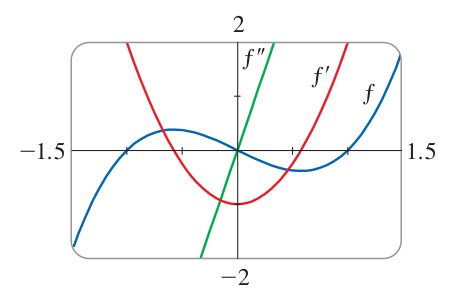
\includegraphics[width=0.55\textwidth]{images/p0195_fig1.png}
    \end{center}

    Chúng ta có thể xem $f''(x)$ là hệ số góc của đường cong $y = f'(x)$ tại điểm $(x, f'(x))$. Nói cách khác, đó là tốc độ thay đổi của hệ số góc của đường cong ban đầu $y = f(x)$.

    Để ý từ Hình 10 rằng $f''(x)$ mang giá trị âm khi $y = f'(x)$ có hệ số góc âm và mang giá trị dương khi $y = f'(x)$ có hệ số góc dương. Do đó đồ thị đóng vai trò như một sự kiểm tra đối với các phép tính của chúng ta.\hfill\textcolor{stewartcyan}{\rule{1.1ex}{1.1ex}}

    \vspace{0.25em}
    Nhìn chung, chúng ta có thể giải thích đạo hàm cấp hai như là tốc độ thay đổi của một tốc độ thay đổi. Ví dụ quen thuộc nhất về điều này là \textit{gia tốc}, được chúng ta định nghĩa như sau.

    Nếu $s = s(t)$ là hàm vị trí của một vật thể chuyển động trên một đường thẳng, ta biết rằng đạo hàm cấp một của nó biểu diễn vận tốc $v(t)$ của vật thể theo thời gian:
    \[
        v(t) = s'(t) = \frac{ds}{dt}
    \]

    Tốc độ thay đổi tức thời của vận tốc theo thời gian được gọi là \textbf{gia tốc} $a(t)$ của vật thể. Như vậy hàm gia tốc là đạo hàm của hàm vận tốc và do đó là đạo hàm cấp hai của hàm vị trí:
    \[
        a(t) = v'(t) = s''(t)
    \]
    \noindent hoặc theo ký hiệu Leibniz,
    \[
        a = \frac{dv}{dt} = \frac{d^2s}{dt^2}
    \]

    Gia tốc là sự thay đổi vận tốc mà bạn cảm nhận được khi tăng tốc hoặc giảm tốc trong ô tô.

    \textbf{Đạo hàm cấp ba} $f'''$ là đạo hàm của đạo hàm cấp hai: $f''' = (f'')'$. Do đó $f'''(x)$ có thể được hiểu là hệ số góc của đường cong $y = f''(x)$ hoặc là tốc độ thay đổi của $f''(x)$. Nếu $y = f(x)$, thì các ký hiệu khác của đạo hàm cấp ba là
    \[
        y''' = f'''(x) = \frac{d}{dx}\left(\frac{d^2y}{dx^2}\right) = \frac{d^3y}{dx^3}
    \]
\end{minipage}
